	The calculations for the bulk band structure are made in the 3D Brillouin zone.
%	The ways of integration in $\kk$-space can be chosen different, but it must be connected. 
	For the calculation of the bulk band structure, we use the following path (like in \cite{tutorial2} p.12)
	\begin{align}
		\text{L} \rightarrow \Gamma \rightarrow \text{X} \rightarrow \text{W} \rightarrow \text{K}
	\end{align} 
	Those symmetry points are illustrated in figure \ref{brillouin_zone} in the theory part. The k-grid and 
%	command for the band structure output is defined in the control.in as
	the command used in order to extract the band structure output from FHI-aims is defined in the control.in file as
	\\
	\begin{minipage}[c]{\linewidth}	\vspace{15pt}
		\begin{verbatim}
		# k_grid settings
		k_grid	24	24	24
		#
		# output band structure
		output band 0.5   0.5   0.5    0.0   0.0   0.0    21  L     Gamma
		output band 0.0   0.0   0.0    0.0   0.5   0.5    21  Gamma X
		output band 0.0   0.5   0.5    0.25  0.5   0.75   21  X     W
		output band 0.25  0.5   0.75   0.375 0.375 0.75   21  W     K
		\end{verbatim} \vspace{0.2cm}
	\end{minipage}
%	The number 21 is the number of $\kk$ points that are computed between two high symmetry points.
	The geometry.in input is the same as the one mentioned in subsection \ref{FHI-aims}. 	
	\begin{figure}[b!]
		\centering
		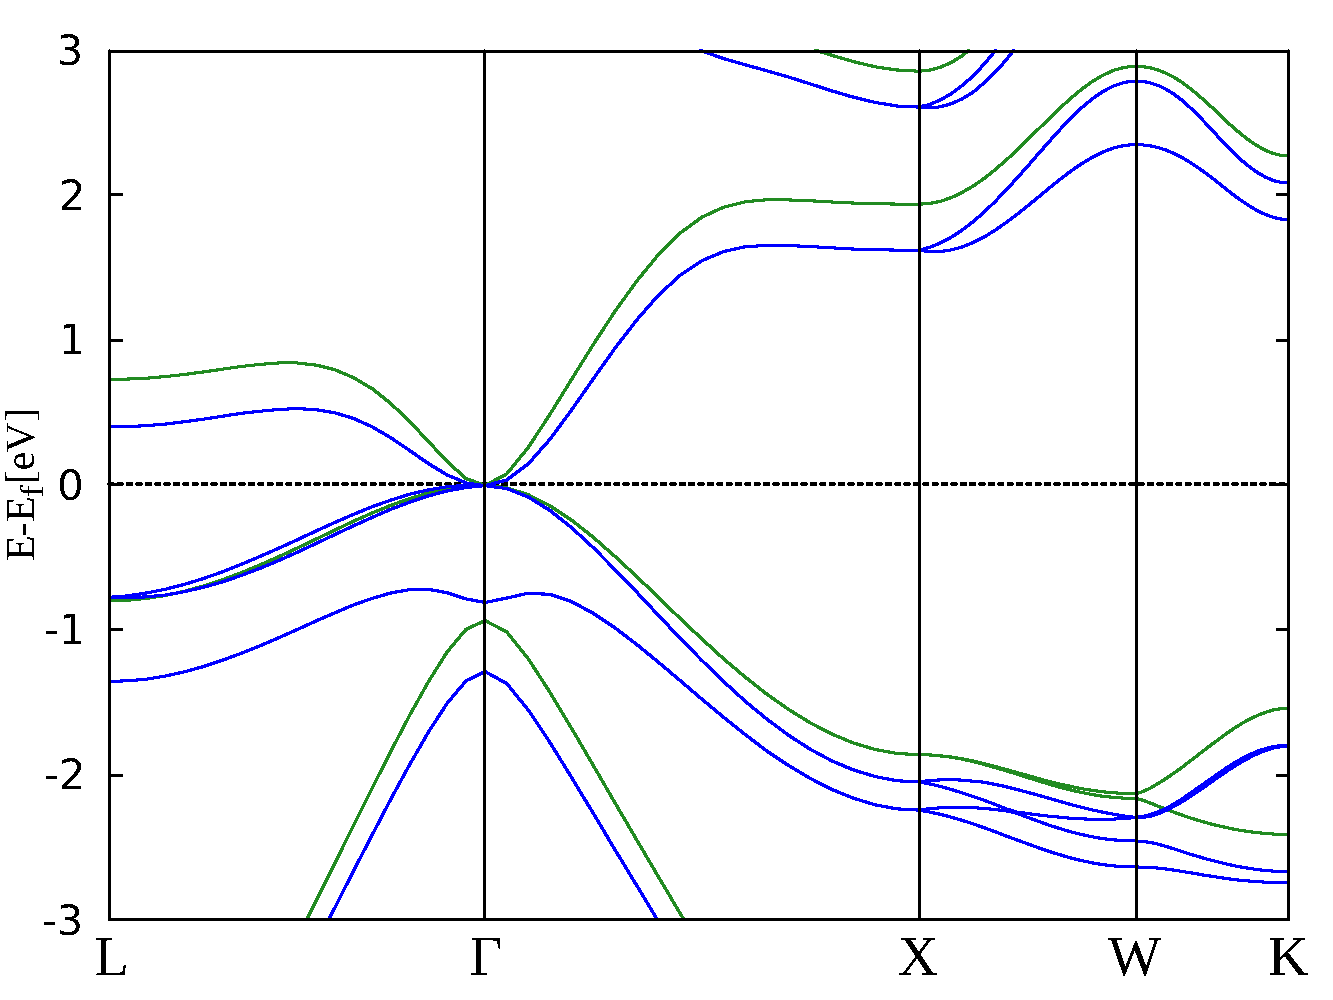
\includegraphics[width=.7\linewidth]{andere_bilder/plot_bulk_with_without_soc.pdf}
		\caption{Band structure of bulk HgTe in the first 3D Brillouin zone. The green lines are the band structure without spin-orbit coupling, and the blue ones include spin-orbit coupling. The Fermi level is indicated by the dashed line.} \label{bulk_band_structure}
	\end{figure}
	
	The outcome of the band structure calculations is shown in figure \ref{bulk_band_structure}, where the green lines indicate the band structure without spin-orbit coupling (SOC) and the blue lines are the calculations with SOC. 
%	Note that the two different band structures just overlap near and at the $\Gamma$ point. 
%%% Local Variables:
%%% mode: latex
%%% TeX-master: "main_BA2.0"
%%% End: